\documentclass[11pt]{beamer}
\usepackage{verbatim}
\usepackage{amsmath}
\usepackage{amsthm}
\usepackage{graphics}
\usepackage{color}
\usepackage{stmaryrd}\usefonttheme[onlymath]{serif}

\title{\textsc{SVMRanker}: A General Termination Aalysis Framework of Loop Programs via SVM\\
Presentation \& Demonstration}
\date{\today}
\author{Xie Li, Yi Li, Yong Li, Xuechao Sun, Andrea Turrini and Lijun Zhang\\ Presentor:}

\newif\ifcomm\commfalse
\begin{document}
\maketitle

\begin{frame}\frametitle{Outline}
\begin{enumerate}
\item Introduction to Ranking Functions 
\item Overview of \textsc{SVMRanker}

\item Demonstration of the Tool in Command Line.
\end{enumerate}

\end{frame}
\begin{frame}\frametitle{Single Path Linear Constraint Loop}{\scriptsize
\begin{example}
\begin{center}

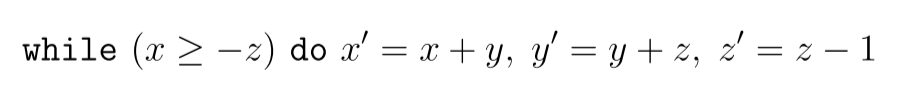
\includegraphics[scale = 0.4]{loopExample.png}


\end{center}


Let $B = (-1, 0, 1)$, $\textbf{x} = (x, y, z)^T, \textbf{b} = 0$.

Let $\textbf{x}'' = (x, y, z, x', y', z')$, 

\begin{equation}
A = \left[
\begin{array}{cccccc}
     1 &1 &0 -1 & 0 & 0 \\
     0 & 1 & 1 & 0 & -1 & 0 \\
     0& 0 & 1 & 0 & 0 & -1
\end{array}
\right]
\end{equation}

and $\textbf{c} = (0, 0, 1)^T$


\end{example}




%\end{frame}
%\begin{frame}\frametitle{Single Path Linear Constraint Loop}
\begin{definition}[SLC]
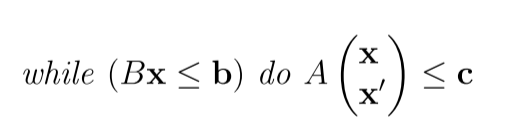
\includegraphics[scale = 0.28]{1.PNG}


\end{definition}
\begin{center}
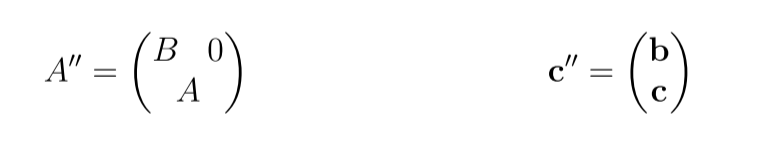
\includegraphics[scale = 0.25]{2.PNG}

$A''\textbf{x}'' \le \textbf{c}''$
\end{center}
}
\end{frame}
\begin{frame}\frametitle{Ranking Functions}

\begin{definition}[Single Linear Ranking Function(LRF)]

$f(x_1, \ldots, x_n) = a_1x_1 + \ldots a_nx_n + a_0$, such that

\begin{itemize}
\item $f(\textbf{x}) \ge 0$ for any $\textbf{x}$ satisfies the loop constraints.

\item $f(\textbf{x}) - f(\textbf{x}') \ge 1$ for any transition from $\textbf{x}$ to $\textbf{x}'$.



\end{itemize}
\end{definition}

\begin{example}
\[\texttt{while }( x - 1 > 0) \texttt{do } x' = x - 5\]

LRF: $f(x) = ax + b$.
\begin{itemize}
\item $ax + b \ge 0$ $\Rightarrow$ $x \ge -\frac{b}{a} = 1$.
\item $ax + b - (ax' + b) = a(x - x') = 5a$ $\Rightarrow$ $5a \ge 1$
\end{itemize}
A possible SLRF: $f(x) = x - 1$
\end{example}

\end{frame}



\begin{frame}\frametitle{Limitation of SLRF}
\[\texttt{while } (q > 0) \texttt{do } q' = q - y, y ' = y + 1\]

Assume there is a LRF for this loop, say $f(q, y) = a_1 q + a_2 y + b$

\[f(q, y) - f(q', y') = a_1y + a_2\]


Since $y$ is not bounded, we cannot guarantee  $\Delta f(q,y,q',y') > 0$

The loop does not has a SLRF, however, it does terminate.

We still wish to use $q$ for ranking function, but to distinguish different ``phase'' of $q$ base on either $y \ge 0$ or $y < 0$ 


\end{frame}
\begin{frame}\frametitle{Nested RF}

\begin{definition}[Nested Ranking Function]

A tuple $\langle f_1, \ldots, f_d\rangle$ is a nested ranking function for $T$ if the following requirements are satisfied for all $\textbf{x}''\in T$
\begin{center}
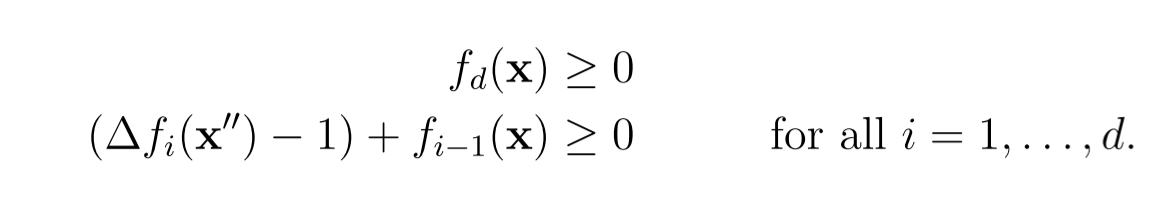
\includegraphics[scale = 0.3]{6.PNG}

\end{center}

Let $f_0 = 0$.
\end{definition}


\end{frame}


\begin{frame}\frametitle{Example: Nested RF}
\begin{center}
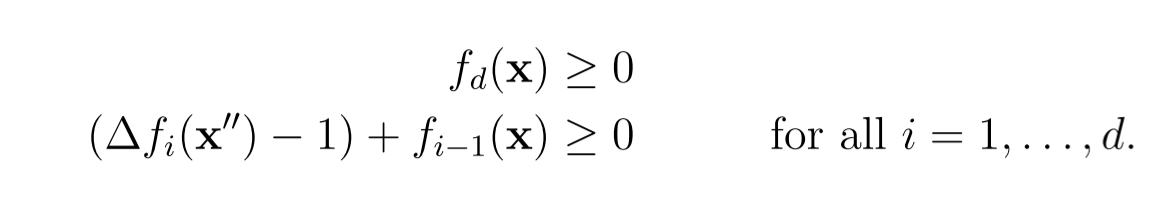
\includegraphics[scale = 0.3]{6.PNG}

\end{center}

\[\texttt{while } (q > 0) \texttt{do } q' = q - y, y ' = y + 1\]

\begin{itemize}
\item Above loop has Nested RF $\langle 1-y, q + 1\rangle$
\item 
\begin{center}
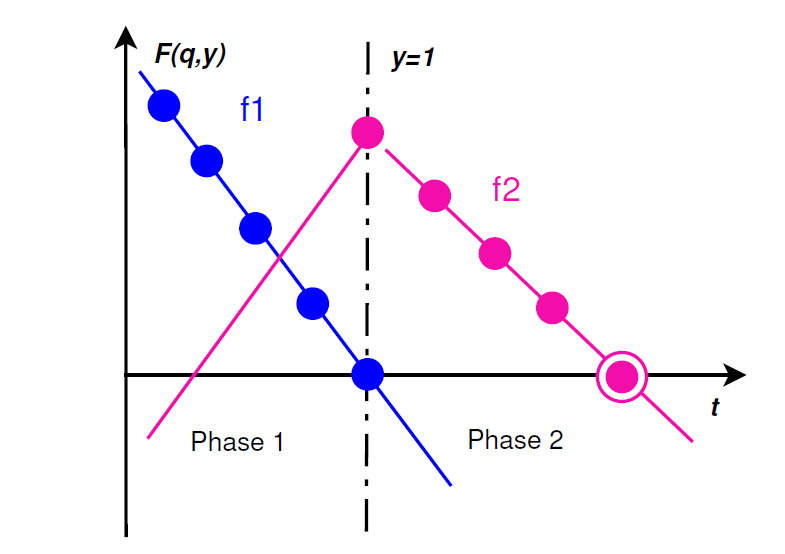
\includegraphics[scale = 0.35]{10.PNG}
\end{center}
\end{itemize}
\end{frame}
\begin{frame}\frametitle{Linear Loop Program}
\begin{definition}
A linear loop program \texttt{LOOP}$(x, x')$ is a binary relation defined by a formula with the free variables $x$ and $x'$ of the form
\begin{center}
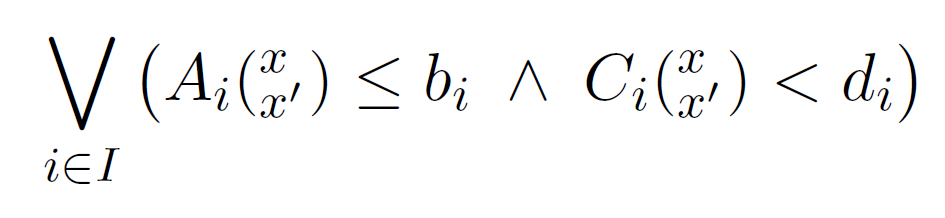
\includegraphics[scale = 0.2]{15.PNG}

\end{center}
for some finite index set $I$.
\end{definition}
\begin{example}
\[\texttt{while } (q > 0)\{\texttt{if } (y > 0): q' = q - y - 1; \texttt{else }: q' = q + y - 1\}\]
can be represented by 
\begin{center}

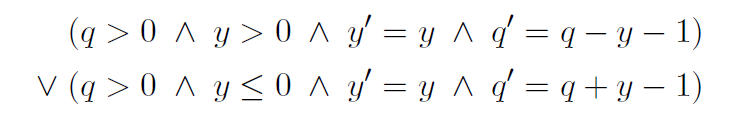
\includegraphics[scale = 0.35]{17.PNG}
\end{center}
\end{example}
\end{frame}
\begin{frame}\frametitle{Limitation of Nested RF}
\begin{example}
\[\texttt{while }(q > 0 \vee y > 0) \]
\[\{\texttt{if }(y > 0): y' = y - 1; q ' = q;\texttt{else }: q' = q - 1\}\]
\end{example}
This program does not have a nested ranking function for we require $f_d\ge 0$ but the guard is $q > 0 \vee y > 0$.

Howerver, this loop does terminate. Then we use a ``multi-phase" ranking function $\langle y,  q\rangle$ to prove the termination.


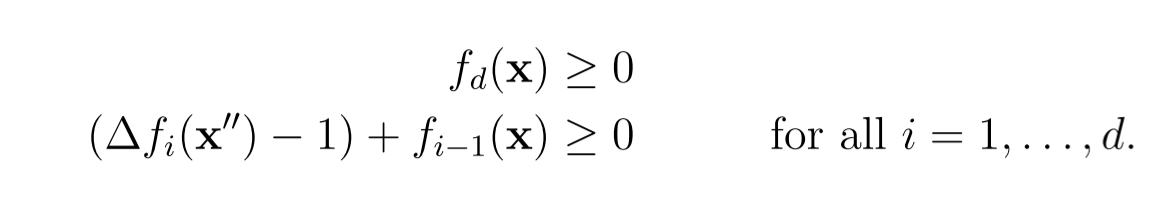
\includegraphics[scale = 0.35]{6.PNG}
\end{frame}



\begin{frame}{Multiphase Ranking Function}
\begin{definition}
Given a set of transitions $T\subseteq \mathbb{Q}^{2n}$, we say $\langle f_1, \ldots, f_d\rangle$ is a multiphase ranking function for $T$ if for every $\textbf{x}'' \in T$, there is an index $i\in [1, d]$, s.t.

\begin{center}
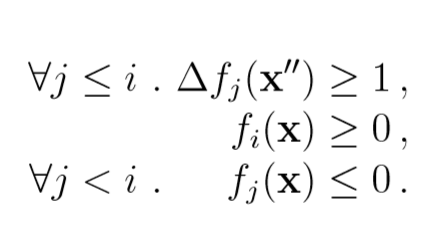
\includegraphics[scale = 0.3]{3.PNG}
\end{center}
We say that $\textbf{x}''$ is ranked by $f_i$(for the minimal).
\end{definition}


\end{frame}


\begin{frame}\frametitle{Example: Multiphase Ranking Function}
\[\texttt{while }( x > -z) \texttt{do } x' = x + y, y' = y + z, z = z - 1\]

Attempt to use a ranking function that has several phases: 
$\langle z + 1, y + 1, x\rangle$
\begin{center}
\begin{tabular}{|c|c|c|c|c|c|}
\hline 
$x$&$y$&$z$&$z+1$&$y+1$&$x$\\
\hline
$1$&$1$&$1$&\textbf{2}&$2$&$1$\\
$2$&$2$&$0$&\textbf{1}&$3$&$2$\\
$4$&$2$&$-1$&\textbf{0}&$3$&$4$\\
\hline
$6$&$1$&$-2$&$-1$&\textbf{2}&$6$\\
$7$&$-1$&$-3$&$-2$&\textbf{0}&$7$\\
\hline
$6$&$-4$&$-4$&$-3$&$-3$&\textbf{6}\\
$2$&$-8$&$-5$&$-4$&$-7$&\textbf{2}\\
\hline
$-6$&$-13$&$-6$&$-5$&$-12$&$-6$\\
\hline
\end{tabular}
\end{center}
\end{frame}
\begin{frame}\frametitle{Example: Multiphase Ranking Function}
\[\texttt{while }( x > -z) \texttt{do } x' = x + y, y' = y + z, z' = z - 1\]
\[\langle z + 1, y + 1, x \rangle\]
$\textbf{x}''$ is ranked by $f_k$ when $i = k$. In this example, $f_1(x, y, z) = z + 1$, $f_2(x, y, z) = y + 1$ and $f_3(x, y, z) = x$
\begin{center}
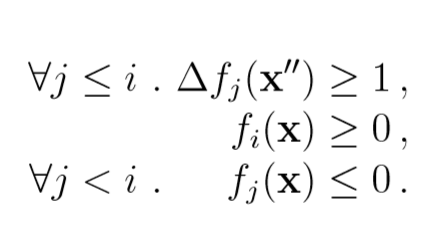
\includegraphics[scale = 0.2]{3.PNG}

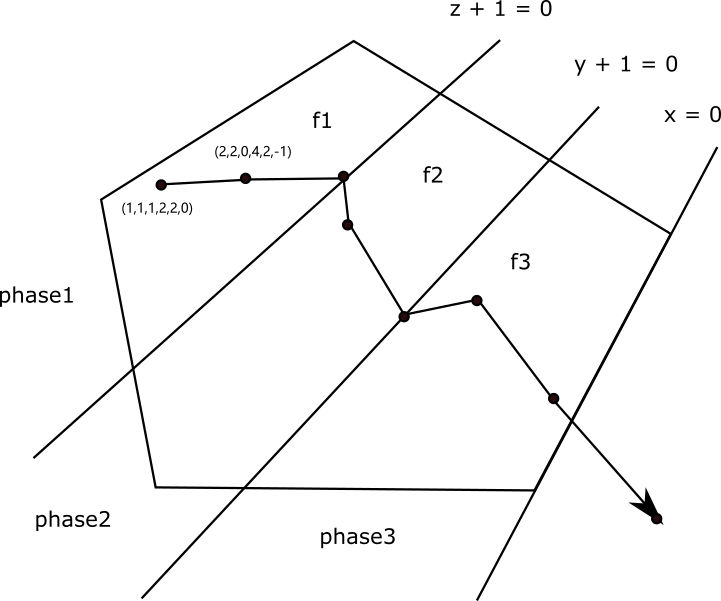
\includegraphics[scale = 0.28]{divide.png}
\end{center}
\end{frame}




\end{document}